\begin{enumerate}[label=\thechapter.\arabic*,ref=\thechapter.\theenumi]

\item An analog signal is sampled at 100 MHz to generate 1024 samples. Only
these samples are used to evaluate 1024-point FFT. The separation between
adjacent frequency points ($\Delta$F) in FFT is \rule{1cm}{0.5mm} kHz.\\
\hfill (GATE BM 2021)\\
\solution
\iffalse
\documentclass[journal,12pt,twocolumn]{IEEEtran}
\usepackage{amsmath,amssymb,amsfonts,amsthm}
\usepackage{txfonts}
\usepackage{tkz-euclide}
\usepackage{listings}
\usepackage{gvv}
\usepackage[latin1]{inputenc}
\usepackage{adjustbox}
\usepackage{array}
\usepackage{tabularx}
\usepackage{pgf}
\usepackage{lmodern}
\usepackage{circuitikz}
\usepackage{tikz}
\usepackage{graphicx}
\usepackage[english]{babel}

\begin{document}
\bibliographystyle{IEEEtran}

\vspace{3cm}

\title{}
\author{EE23BTECH11047 - Deepakreddy P
}
\maketitle
\newpage
\bigskip

\noindent \textbf{32} \quad An analog signal is sampled at 100 MHz to generate 1024 samples. Only
these samples are used to evaluate 1024-point FFT. The separation between
adjacent frequency points ($\Delta$F) in FFT is \rule{1cm}{0.5mm} kHz.\\
\hfill (GATE BM 2021)\\
\solution
\fi

\begin{center}
    \begin{table}[ht]
        \setlength{\arrayrulewidth}{0.3mm}
\setlength{\tabcolsep}{12pt}
\renewcommand{\arraystretch}{1.3}


\begin{center}
\caption{Input Parameters}
\begin{tabular}{ |p{1.7cm}|p{1.7cm}|p{1.7cm}|  }

\hline
 {Symbol}&{Description} & {value}\\
\hline
$f_s$ & Sampling frequency & 100 MHz\\
\hline
$N$ & No of samples  & 1024\\
\hline

\end{tabular}
\end{center}

    \end{table}
\end{center}

\begin{align}
    \Delta F &= \frac{f_s}{N}\\
    \Delta F &= \frac{100}{1024} MHz\\
    \Delta F &= \frac{10^5}{1024} kHz\\
    \Delta F &= 97.66kHz
\end{align}


\begin{figure}[ht]
   \centering
   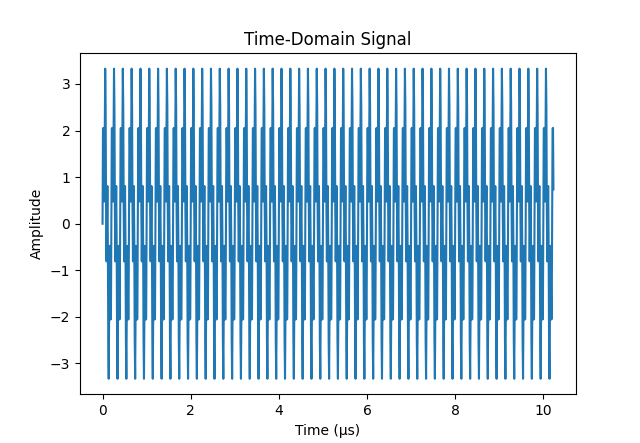
\includegraphics[width=1.1\columnwidth]{2021/BM/32/figs/fig1.png}
   \caption{Time Domain Signal}
\end{figure}

\begin{figure}[ht]
   \centering
   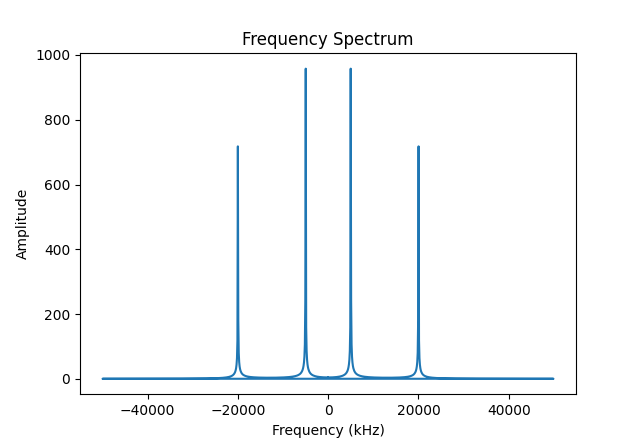
\includegraphics[width=1.1\columnwidth]{2021/BM/32/figs/fig2.png}
   \caption{Frequency Spectrum}
\end{figure}






%\end{document}


\newpage

\item Consider a real-valued base-band signal $x(t)$, band limited to $10kHz$. The Nyquist rate for the signal \\\\
$y(t) = x(t)x(1+\dfrac{t}{2})$ is\\

\begin{enumerate}
\item[(A)] $15kHz$
\item[(B)] $30kHz$
\item[(C)] $60kHz$
\item[(D)] $20kHz$
\end{enumerate}
\hfill{(GATE EC 2021)}\\
\solution
\let\negmedspace\undefined
\let\negthickspace\undefined
\documentclass[journal,12pt,twocolumn]{IEEEtran}
\usepackage{cite}
\usepackage{amsmath,amssymb,amsfonts,amsthm}
\usepackage{algorithmic}
\usepackage{graphicx}
\usepackage{textcomp}
\usepackage{xcolor}
\usepackage{txfonts}
\usepackage{listings}
\usepackage{enumitem}
\usepackage{mathtools}
\usepackage{gensymb}
\usepackage{comment}
\usepackage[breaklinks=true]{hyperref}
\usepackage{tkz-euclide}
\usepackage{listings}
\usepackage{gvv}
\def\inputGnumericTable{}
\usepackage[latin1]{inputenc}
\usepackage{color}
\usepackage{array}
\usepackage{longtable}
\usepackage{calc}
\usepackage{multirow}
\usepackage{hhline}
\usepackage{ifthen}
\usepackage{lscape}
\usepackage{circuitikz}

\newtheorem{theorem}{Theorem}[section]
\newtheorem{problem}{Problem}
\newtheorem{proposition}{Proposition}[section]
\newtheorem{lemma}{Lemma}[section]
\newtheorem{corollary}[theorem]{Corollary}
\newtheorem{example}{Example}[section]
\newtheorem{definition}[problem]{Definition}
\newcommand{\BEQA}{\begin{eqnarray}}
\newcommand{\EEQA}{\end{eqnarray}}
\newcommand{\define}{\stackrel{\triangle}{=}}
\theoremstyle{remark}
\newtheorem{rem}{Remark}
\begin{document}

\bibliographystyle{IEEEtran}
\vspace{3cm}

\title{Gate 2021- Instrumentation Engineering}
\author{EE23BTECH11058 - Sindam Ananya$^{*}$% <-this % stops a space
}
\maketitle
\newpage
\bigskip

\renewcommand{\thefigure}{\theenumi}
\renewcommand{\thetable}{\theenumi}

\vspace{3cm}
\textbf{Question 43:} 
Given $y(t) = e^{-3t}u(t) * u(t+3)$, where * denotes convolution operation. The value of $y(t)$ as $t \rightarrow \infty$ is
\hfill{(GATE IN 2021)}\\
\solution
\begin{align}
y(t) &=  e^{-3t}u(t) * u(t+3)\\
x(t) &\xleftrightarrow{\mathcal{L}} X(s)\\
x(t-t_o) &\xleftrightarrow{\mathcal{L}} e^{-s t_o}X(s)\\
x_1(t) * x_2(t) &\xleftrightarrow{\mathcal{L}} X_1(s)X_2(s)\\
e^{-at}u(t) &\xleftrightarrow{\mathcal{L}} \frac{1}{s + a} \quad \brak{ROC:Re(s)>-a}\\
u(t) &\xleftrightarrow{\mathcal{L}} \frac{1}{s} \quad \brak{ROC:Re(s)>0}\\
u(t+3) &\xleftrightarrow{\mathcal{L}} \frac{e^{3s}}{s} \quad \brak{ROC:Re(s)>0}\\ 
Y(s) &= \brak{\frac{1}{s + 3}}\brak{\frac{e^{3s}}{s}} \quad \brak{ROC:Re(s)>0}
\label{eq:gate202143}
\end{align}
By using Final Value Theorem,
\begin{align}
\lim\limits_{t \to \infty} y(t) &= \lim\limits_{s \to 0} sY(s)\\
                                &= \lim\limits_{s \to 0} s\brak{\frac{1}{s + 3}}\brak{\frac{e^{3s}}{s}}\\
                                &= \frac{1}{3}
\end{align}
By solving the equation \eqref{eq:gate202143} through partial fractions,
\begin{align}
Y(s) = \frac{e^{3s}}{3s} - \frac{e^{3s}}{3\brak{s+3}} 
\end{align}
By applying inverse laplace transform,
\begin{align}
y(t) = \frac{u(t+3)}{3} - \frac{e^{-3(t+3)}u(t+3)}{3}
\end{align}
\begin{figure}[h!]
    \centering
    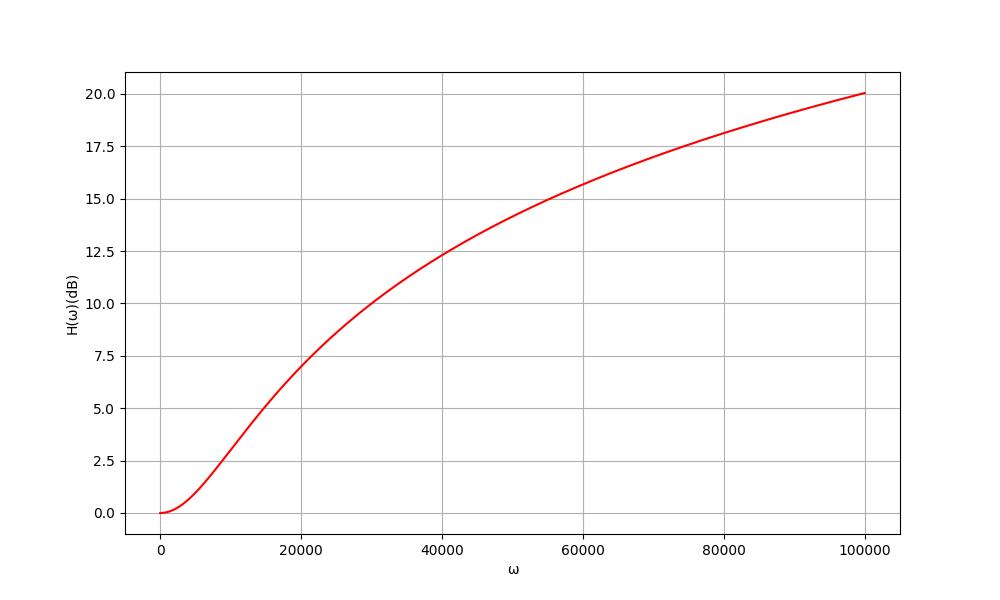
\includegraphics[width=0.8\columnwidth]{figs/plot.png}
    \caption{plot of $y(t)$}
    \label{fig:gate202138fig}
\end{figure}
\end{document}

\newpage
\item A continous time transfer function, $\text{H\brak{\text{s}}}=\frac{1+\frac{\text{s}}{10^6}}{\text{s}}$ is coverted to a discrete time transfer function, $\text{H\brak{\text{z}}}$ using a bi-linear transformation at 100 MHz sampling rate. The pole of $\text{H\brak{\text{z}}}$ is located at z = ?\hfill \brak{\text{GATE BM 2021}}\\

\solution
\input{2021/BM/22/gate,2k21,bm22.tex}
\newpage

\item 	A 4 kHz sinusoidal message signal having amplitude 4 V is fed to a delta modulator (DM) operating at a sampling rate of 32 kHz. The minimum step size required to avoid slope overload noise in the DM is?
\hfill{(GATE EC 2021)}
\solution
\iffalse
\let\negmedspace\undefined
\let\negthickspace\undefined
\documentclass[journal,12pt,onecolumn]{IEEEtran}
\usepackage{cite}
\usepackage{amsmath,amssymb,amsfonts,amsthm}
\usepackage{algorithmic}
\usepackage{graphicx}
\usepackage{textcomp}
\usepackage{xcolor}
\usepackage{txfonts}
\usepackage{listings}
\usepackage{enumitem}
\usepackage{mathtools}
\usepackage{gensymb}
\usepackage{comment}
\usepackage[breaklinks=true]{hyperref}
\usepackage{tkz-euclide} 
\usepackage{listings}
\usepackage{gvv}                                        
\def\inputGnumericTable{}                                 
\usepackage[latin1]{inputenc}                                
\usepackage{color}                                            
\usepackage{array}                                            
\usepackage{longtable}                                       
\usepackage{calc}                                             
\usepackage{multirow}                                         
\usepackage{hhline}                                           
\usepackage{ifthen}                                           
\usepackage{lscape}
\usepackage{siunitx}
\usepackage{flushend}
\usepackage[siunitx]{circuitikz}
\usepackage{caption}
\usepackage{setspace}

\newtheorem{theorem}{Theorem}[section]
\newtheorem{problem}{Problem}
\newtheorem{proposition}{Proposition}[section]
\newtheorem{lemma}{Lemma}[section]
\newtheorem{corollary}[theorem]{Corollary}
\newtheorem{example}{Example}[section]
\newtheorem{definition}[problem]{Definition}
\newcommand{\BEQA}{\begin{eqnarray}}
	\newcommand{\EEQA}{\end{eqnarray}}
\newcommand{\define}{\stackrel{\triangle}{=}}
\theoremstyle{remark}
\newtheorem{rem}{Remark}
\begin{document}
	
	\bibliographystyle{IEEEtran}
	\vspace{3cm}
	
	\title{GATE 2021 EC.24}
	\author{EE23BTECH11203 - Adarsh A$^{*}$% <-this % stops a space
	}
	\maketitle
	%\newpage
	\bigskip
	
	\renewcommand{\thefigure}{\theenumi}
	\renewcommand{\thetable}{\theenumi}
	
	
	\vspace{0.2cm}
	\linespread{1.1}
	%\onehalfspacing
	
	%\fontsize{14}{20}\selectfont
	\textbf{Question : }
	A 4 kHz sinusoidal message signal having amplitude 4 V is fed to a delta modulator (DM) operating at a sampling rate of 32 kHz. The minimum step size required to avoid slope overload noise in the DM is?
	
	\vspace{0.3cm}
	\solution
 	\fi
	
	\begin{table}[htbp]
	\centering
	\noindent
	\fontsize{10}{15}\selectfont {
		\resizebox{0.6\textwidth}{!}{%
			\begin{tabular}{|c|c|c|}
				\hline
				\textbf{Parameter} & \textbf{Value} & \textbf{Description} \\
				\hline
				$\delta$ & - & Step size \\
				\hline
				$f_s$ & 32 kHz & Sampling rate \\
				\hline
				$A_{max}$ & 4 V & Maximum amplitude of message signal  \\
				\hline
				$f_m$ & 4 kHz & Frequency of message signal  \\
				\hline
			\end{tabular}
	} }
	\caption{Input Table}
	
\end{table}

	
	To avoid slope overload distortion,
	\begin{align}
		\delta f_s &\geq 2\pi A_{max} f_m
	\end{align}
	
	The minimum slope can be obtained when,
	\begin{align}
		\delta_{min} f_s &= 2\pi A_{max} f_m\\
		\delta_{min} \brak {32} &= 2\pi \brak 4 \brak 4\\
		\delta_{min} &= \pi
	\end{align}
	
	\begin{figure}[htbp]
		\centering
		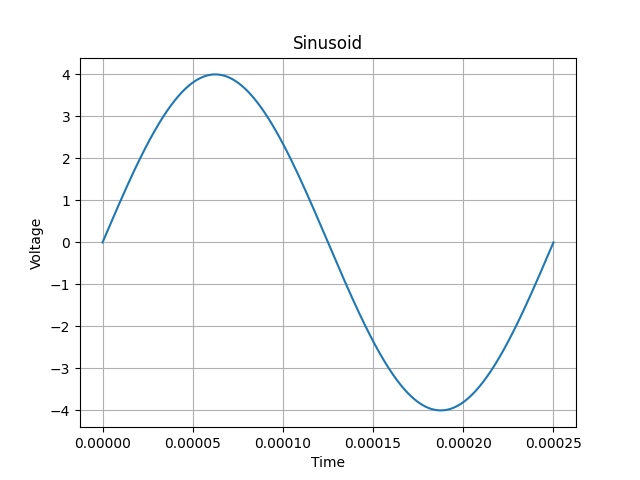
\includegraphics[width=0.7\textwidth]{2021/EC/24/figs/Figure_2.png}
		\caption{(a) Plot of the sinusoid}
	\end{figure}
	
	\begin{figure}[htbp]
		\centering
		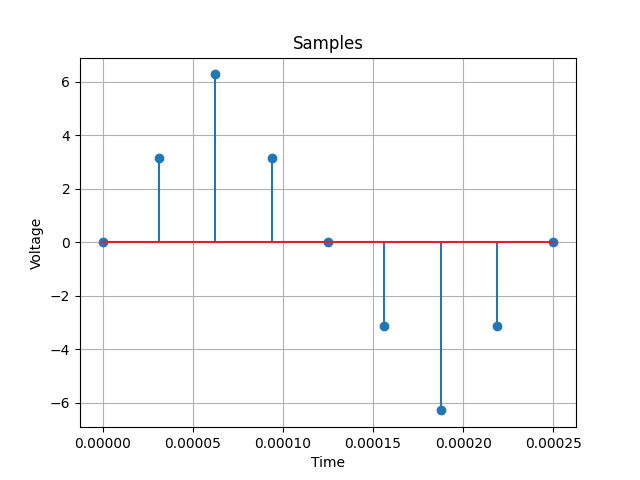
\includegraphics[width=0.7\textwidth]{2021/EC/24/figs/Figure_1.png}
		\caption{(b) Plot of the samples with $\delta_{min}$}
	\end{figure}
%\end{document}

\newpage

\end{enumerate}
